%%%%%%%%%%%%%%%%%%%%%%%%
%
% $Author: Deepti Hegde $
% $Datum: 2023-06-25  $
% $Pfad: BA23-02-Sales-Predictor/report/Contents/en/Introduction.tex $
% $Version: 1.0 $
% $Reviewed by: Deepti, Sadegh and Raunak $
% $Review Date: 2023-06-30 $
%
%%%%%%%%%%%%%%%%%%%%%%%%



\chapter{Deployment}

\section{User Interface}

\subsection{Writing the Code}

We generated forecasts using multiple machine learning models. The code for analysing and predicting the data was written in PyCharm. Different packages were installed in PyCharm to write the required code.The general packages were Pandas, Numpy. Pandas help in data analysis by importing and manipulating data. Numpy is useful if we want to use mathematical functions.For checking stationarity statsmodels.api was used. Data visualisation was acheivedusing matplotlib.pyplot package.Validation metrics were generated by using sklearn.metrics and numpy.

\subsection{PyCharm}

PyCharm is an \ac{ide} for Python that is widely used by developers for building software applications, including machine learning projects. PyCharm is known for its ease of use, extensive feature set, and powerful tools for code analysis and debugging. Here are some of the usability features that make PyCharm an excellent choice for Python-based machine learning projects:

\begin{itemize}

\item Intuitive interface: PyCharm has a user-friendly interface that makes it easy to navigate and use. The IDE has a clean layout that includes useful tools like a code editor, a project navigator, a debugger, and a terminal.

\item Code completion and error detection: PyCharm includes intelligent code completion and error detection features that can save you time and effort when writing code. The IDE can suggest code snippets, variable names, and function definitions as you type, and it can highlight errors and suggest fixes in real-time.

\item Integrated debugging: PyCharm has a built-in debugger that makes it easy to identify and fix errors in your code. You can set breakpoints, step through code, and inspect variables and data structures in real-time.

\item Integration with popular machine learning libraries: PyCharm supports popular machine learning libraries like TensorFlow, PyTorch, and scikit-learn, providing a seamless integration between the IDE and these libraries.

\item Version control integration: PyCharm integrates with popular version control systems like Git, allowing you to manage your code and collaborate with others easily.

\item Customization: PyCharm allows you to customize the IDE to your liking by adjusting the color scheme, key bindings, and other preferences.

\end{itemize}


\section{Structure and Idea}

	The purpose of this report is to outline the process of developing a sales prediction model using the XGBoost algorithm. This chapter provides an overview of the documentation structure, the idea behind the project, the flowchart of the implementation, and the machine learning pipeline employed.
	
	The documentation for this sales prediction project follows a structured approach to ensure clarity and ease of understanding. It provides a brief overview of the project's objective and contents of the report. Describes the process of acquiring and preparing the dataset for analysis. In addition to that, explains the techniques used and the steps involved in training and evaluating the XGBoost model.
	
	The main \textbf{idea} of this project is to create a machine learning model that can predict sales reliably based on previous data and pertinent attributes. We intend to construct a robust and reliable sales prediction model by leveraging the XGBoost algorithm, which is well-known for its ability in dealing with structured data and gradient boosting.
	
	\subsection{Flow chart}
	
	The flow chart below illustrates the high-level process of developing the sales prediction model using XGBoost starting from data collection to model evaluation.
	
	\begin{center}
		\begin{figure}[H]
			\begin{center}
				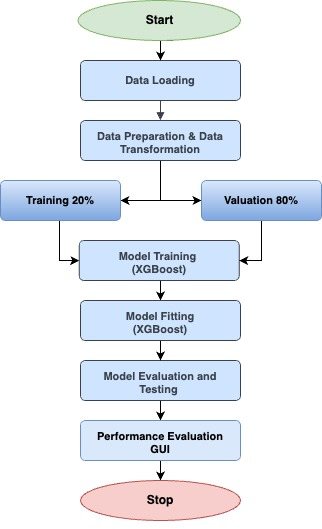
\includegraphics[height=125mm, width=130mm]{Images/DevelopmentFlowChart}
			\end{center}
			\caption{ XGBoost Development FlowChart}
		\end{figure}
	\end{center}

\section{ML Pipeline}
	
	The deployment stage of the KDD process for sales forecasting involves the deployment of the predictive models generated in the data mining stage. To estimate future sales, we used a variety of regression algorithms in this project, including Linear Regression, DecisionTree Regressor, ExtraTrees Regressor, Random Forest Regressor, Gradient Boosting Regressor, and XGBOOST.\bigskip
	
	To choose the top-performing algorithm before deploying these models, we first assessed each one's performance on a test dataset. \ac{MAE}, \ac{MSE} and \ac{R2} score were the evaluation metrics employed. We chose the optimum algorithm for deployment based on the evaluation findings.\bigskip
	
	We got the highest R2 score 0.858251 and 0.00013143 MSE score using XGBOOST algorithm. The second highest R2 score is 0.83944 from the Random Forest Regressor and Gradient Boosting Regressor algorithms.

\begin{itemize}
	
	\item Data Collection: 
	
	Collect historical sales data, including important elements such as product information, time series data, and external factors that may influence sales.
	
	\item Data Preprocessing: 
	
	Remove missing values, outliers, and formatting errors from the data. If necessary, perform feature scaling or normalization.
	
	\item Feature Engineering: 
	
	Use techniques such as one-hot encoding, feature extraction, or establishing lag variables to transform raw data into meaningful features.
	
	\item Model Training: 
	
	Train the XGBoost model using the training set. This involves fitting the model to the training data and optimizing the model's hyperparameters to find the best combination for your specific problem. The XGBoost algorithm utilizes gradient boosting to iteratively improve the model's predictions.
	
	\item Model Evaluation: 
	
	Use appropriate evaluation measures to assess the model's performance, such as mean squared error (MSE), root mean squared error (RMSE), or R-squared value. If necessary, fine-tune the model.
	
	\item Prediction: 
	
	Deploy the trained model to make predictions on new, unseen data to estimate future sales.
	
\end{itemize}

\begin{center}
	\begin{figure}[h!]
		\begin{center}
			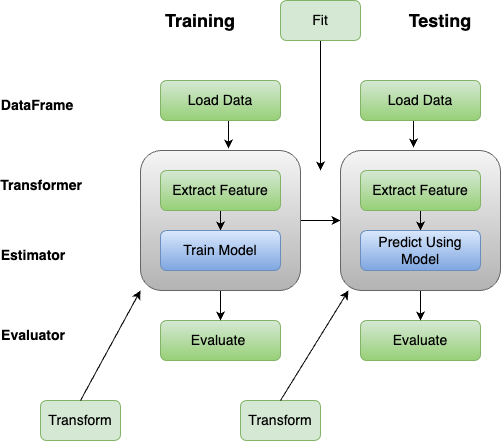
\includegraphics[height=90mm, width=130mm]{Images/MLPipeline}
		\end{center}
		\caption{ ML Pipeline for Sales Prediction}
	\end{figure}
\end{center}
